%% Andrea Di Iorio - 277550 -  SpMV - SCPA - 
%% tex template from `docstrip(samples.dtx,`acmsmall') -> sample-acmsmall.tex'
%% main package get: https://www.ctan.org/pkg/acmart
%% Commands for TeXCount
%TC:macro \cite [option:text,text]
%TC:macro \citep [option:text,text]
%TC:macro \citet [option:text,text]
%TC:envir table 0 1
%TC:envir table* 0 1
%TC:envir tabular [ignore] word
%TC:envir displaymath 0 word
%TC:envir math 0 word
%TC:envir comment 0 0


\documentclass[acmsmall,nonacm=true]{acmart}
%%nonacm to avoid banners and other template stuff

%\newcommand{\vvv}[1]{\verbatim{#1} }
\newcommand{\vvv}[1]{{\small\texttt{#1}}}
%%CODE EMBEDD 
\usepackage{listings,color}  
%CONFIG CODE LISTINGS 
\definecolor{mygreen}{rgb}{0,0.6,0}       
\definecolor{mygray}{rgb}{0.5,0.5,0.5}    
\definecolor{mymauve}{rgb}{0.58,0,0.82}   
 
\lstloadlanguages{C} 
\lstdefinestyle{C_typedefs}{ 
  language=C, 
  keywordstyle=\color{red}, 
  morekeywords={uint,ulong},
  morecomment=[l][\color{purple}]{\#pragma}
} 
\lstset{ 
  %escapechar=\%,                  %%EMBEDD LATEX CODE IN SOURCE CODE 
  escapeinside={*@}{@*},       %%EMBEDD LATEX CODE IN SOURCE PARTI RACCHIUSE DA QUESTE DUE COPPIE              
  captionpos=b,                    % sets the caption-position to bottom 
  tabsize=2,                       % sets default tabsize to 2 spaces 
  %title=\lstname                   % show the filename of files included with \lstinputlisting; also try caption instead of title 
  basicstyle=\footnotesize,        % the size of the fonts that are used for the code 
  basewidth=0.6em,   fontadjust=true, %fontSizes config in manual 
  numberstyle=\tiny, % the style that is used for the line-numbers 
  numbersep=3pt,                   % how far the line-numbers are from the code 
  numbers=left,                    % where to put the line-numbers; possible values are (none, left, right) 
  numberfirstline=true,   firstnumber=1, 
  stepnumber=1,                    % the step between two line-numbers. If it's 1, each line will be numbered 
  frame=lines,                   % bordo attorno al codice 
  keepspaces=true,                 % keeps spaces in text, useful for keeping indentation of code (possibly needs columns=flexible) 
  keywordstyle=\color{red},       % keyword style 
  language=C,             % the language of the code 
  style=C_typedefs, 
  %deletekeywords={...},            % if you want to delete keywords from the given language 
  rulecolor=\color{black},         % if not set, the frame-color may be changed on line-breaks within not-black text (e.g. comments (green here)) 
  showspaces=false,                % show spaces everywhere adding particular underscores; it overrides 'showstringspaces' 
  showstringspaces=false,          % underline spaces within strings only 
  showtabs=false,                  % show tabs within strings adding particular underscores 
  backgroundcolor=\color{white},   % choose the background color; you must add \usepackage{color} or \usepackage{xcolor}; should come as last argument 
  breakatwhitespace=false,         % sets if automatic breaks should only happen at whitespace 
  breaklines=true,                 % sets automatic line breaking 
  commentstyle=\color{mygreen},    % comment style 
  extendedchars=false,             % lets you use non-ASCII characters; for 8-bits encodings only, does not work with UTF-8 
  stringstyle=\color{mymauve},     % string literal style 
} 


%% \BibTeX command to typeset BibTeX logo in the docs TODO REMOVE
\AtBeginDocument{%
  \providecommand\BibTeX{{%
    \normalfont B\kern-0.5em{\scshape i\kern-0.25em b}\kern-0.8em\TeX}}}

%%% Rights management information.  This information is sent to you
%%% when you complete the rights form.  These commands have SAMPLE
%%% values in them; it is your responsibility as an author to replace
%%% the commands and values with those provided to you when you
%%% complete the rights form.
%\setcopyright{acmcopyright}
%\copyrightyear{2018}
%\acmYear{2018}
%\acmDOI{10.1145/1122445.1122456}
%
%
%%%
%%% These commands are for a JOURNAL article.
%\acmJournal{JACM}
%\acmVolume{37}
%\acmNumber{4}
%\acmArticle{111}
%\acmMonth{8}

%%
%% Submission ID.
%% Use this when submitting an article to a sponsored event. You'll
%% receive a unique submission ID from the organizers
%% of the event, and this ID should be used as the parameter to this command.
%%\acmSubmissionID{123-A56-BU3}

%%
%% The majority of ACM publications use numbered citations and
%% references.  The command \citestyle{authoryear} switches to the
%% "author year" style.
%%
%% If you are preparing content for an event
%% sponsored by ACM SIGGRAPH, you must use the "author year" style of
%% citations and references.
%% Uncommenting
%% the next command will enable that style.
%%\citestyle{acmauthoryear}

\begin{document}

% "title"  + shortTitle
% \title [SpMV in OMP e CUDA] {SpMV - Implementazioni OMP e CUDA}
\title {SpMV - Implementazioni OMP e CUDA}

%%
%% The "author" command and its associated commands are used to define
%% the authors and their affiliations.
%% Of note is the shared affiliation of the first two authors, and the
%% "authornote" and "authornotemark" commands
%% used to denote shared contribution to the research.

\author{Andrea Di Iorio}
%\authornote{Both authors contributed equally to this research.}
%\email{trovato@corporation.com}
%\orcid{0277550}
%\affiliation{%
%  \institution{ Torvergata }
%  \streetaddress{P.O. Box 1212}
%  \city{Dublin}
%  \state{Ohio}
%  \country{USA}
%  \postcode{43017-6221}
%}
\authorsaddresses{}	%force empty address overriding

%%
%% By default, the full list of authors will be used in the page
%% headers. Often, this list is too long, and will overlap
%% other information printed in the page headers. This command allows
%% the author to define a more concise list
%% of authors' names for this purpose.
\renewcommand{\shortauthors}{Andrea Di Iorio}

\begin{abstract}
Il progetto consiste in varie implementazioni del nucleo di calcolo
$y \leftarrow A~x$ ovvero il prodotto di una matrice sparsa con un vettore.
Questa operazione è essenziale per la soluzione di sistemi lineari sparsi 
ed è estremamente importante per varie applicazioni di calcolo scientifico.\\ %e egenvalue problems solved by iterative methods
Nel seguito si farà riferimento a matrici sparse di \vvv{M} righe e \vvv{N} colonne con
in numero massimo di non zeri nelle varie righe pari ad \vvv{MAX\_NZ\_ROW}
\end{abstract}

%%%
%%% The code below is generated by the tool at http://dl.acm.org/ccs.cfm.
%%% Please copy and paste the code instead of the example below.
%%%
%\begin{CCSXML} ....  reliability

\keywords{SpMV, CSR 2D partitioning, sparse linear sistems, HPC, scientific computing}

\settopmatter{printacmref=false,printfolios=true}

%%
%% This command processes the author and affiliation and title
%% information and builds the first part of the formatted document.
\maketitle


%%%%RELAZIONE
Segue una descrizione delle implementazioni realizzate per risolvere
il problema in oggetto

\section{Implementazioni OpenMP}
\subsection{CSR}
\subsubsection{Partizionamento monodimensionale della matrice}\hfill\\	%TODO bf
Semplici implementazioni per SpMV si possono ottenere effettuando una
parallelizzazione su (blocchi di) righe della matrice sparsa, 
delegando ad ogni thread l'accumulazione del prodotto punto tra 
la riga della matrice assegnatagli e il vettore in ingresso.
\label{spmvRowsBlocksCSR}
\begin{lstlisting} 
#pragma omp parallel for schedule(runtime) private(acc,block,startRow,c)
for (ulong b=0;   b<cfg->gridRows;   b++){
    block      = UNIF_REMINDER_DISTRI(b,rowBlock,rowBlockRem);
    startRow   = UNIF_REMINDER_DISTRI_STARTIDX(b,rowBlock,rowBlockRem);
    for (ulong r=startRow;  r<startRow+block;  r++){
        acc = 0;
        #if SIMD_ROWS_REDUCTION == TRUE
        #pragma omp simd reduction(+:acc)
        #endif
        for (ulong j=mat->IRP[r]; j<mat->IRP[r+1]; j++){
           c = mat->JA[j];
           acc += mat->AS[j] * vect[c];
        }
        outVect[r] = acc;
    } 
}
\end{lstlisting}
Nello snippet di codice precedente, appartenente alla funzione \vvv{spmvRowsBlocksCSR},
si parallelizza il calcolo di SpMV in blocchi
di righe di dimensione pari al numero di righe diviso il valore 
all'interno del campo \vvv{gridRows}.\\
\label{UNIF_REMINDER_DISTRI}
Questi blocchi hanno una dimensione il più possibile simile per migliorare
l'uniformità dei lavori assegnati ai thread e quindi minimizzare il divario nel
loro tempo di completamento, nell'ipotesi di avere un carico di lavoro uniforme per ogni
blocco di righe.
Grazie all'uso delle macro \vvv{UNIF\_REMINDER\_DISTRI} e \vvv{UNIF\_REMINDER\_DISTRI\_STARTIDX},
viene ridistribuito il resto della divisione tra il numero di righe della
matrice e la variabile \vvv{gridRows} tra tutti i thread.\\

Un altro partizionamento monodimensionale è realizzato dalla
funzione \vvv{spmvRowsBasicCSR}, dove si suddividono tutte le righe della matrice
tra i thread disponibili in base allo scheduling e il chunk configurato nel \vvv{\#pragma omp parallel for}.

\subsubsection{Partizionamento 2D della matrice} \label{CSR_2D}\hfill\\	%TODO bf
Effettuando un partizionamento bidimensionale della matrice in ingresso è
possibile assegnare ad ogni thread un blocco di dati con cui accumulare un prodotto
punto parziale tra il vettore e porzioni di righe.\\
Successivamente mediante
operazioni di riduzione è possibile avere i risulati finali dei prodotti punto e
quindi il vettore risultante all'operazione di SpMV.\\

\label{spmvTilesCSR}
\begin{lstlisting} 
#pragma omp parallel for schedule(runtime) private(acc,rowBlock,startRow,c,t_i,t_j)
for (ulong tileID = 0; tileID < gridSize; tileID++){
    ///get iteration's indexing variables
    t_i = tileID/cfg->gridCols;  //i-th row block
    t_j = tileID%cfg->gridCols;  //j-th col block
    //get tile row-cols group FAIR sizes
    rowBlock = UNIF_REMINDER_DISTRI(t_i,_rowBlock,_rowBlockRem); 
    startRow = UNIF_REMINDER_DISTRI_STARTIDX(t_i,_rowBlock,_rowBlockRem);

    for (ulong r=startRow,partOffID;  r<startRow+rowBlock;  r++){
        partOffID = IDX2D(r,t_j,cfg->gridCols);
        acc = 0;
        #if SIMD_ROWS_REDUCTION == TRUE
        #pragma omp simd reduction(+:acc)
        #endif
        //2D CSR tile SpMV using cols partition of row r
        for (ulong j=offsets[partOffID]; j<offsets[partOffID+1]; j++){
            c = mat->JA[j];
            acc += mat->AS[j] * vect[c]; 
        }
        tilesOutTmp[partOffID] = acc;
    }
}
for (ulong r=0;  r<mat->M;   r++){
    for (ulong p=0;   p<cfg->gridCols;   p++){
        outVect[r] += tilesOutTmp[ IDX2D(r,p,cfg->gridCols) ];
    }
}
\end{lstlisting}
%%//#pragma omp parallel for reduction(+:outVect[:mat->M])    //TODO RARE SEGFAULT
Nello snippet di codice precedente, appartenete alla funzione \vvv{spmvTilesCSR},
si assegna ad ogni thread un blocco della matrice di dimensione pari ad una
suddivisone del numero di colonne e di righe rispettivamente per i campi 
\vvv{gridCols} e \vvv{gridRows}.\\
Mediante le variabili \vvv{t\_i, t\_j}, si identifica una partizione CSR delle colonne
della matrice ed un blocco di righe al suo interno su cui effettuare i prodotti
punti parziali per SpMV, seguiti poi da un operazione di riduzione da riga 23.\\
\label{CSR_2D_PARTITIONING}
\subsubsection{metodologie di partizionamento 2D di una matrice CSR}\hfill\\ %TODO subsubsection
Il partizionamento bidimensionale di una matrice sparsa in formato CSR è
realizzabile mediante una suddivisione delle colonne della matrice che possono essere
accedute come sottomatrici CSR salvate separatamente \label{spmvTilesAllocdCSR}
o con riferimenti in una struttura ausiliaria. 
Quest'ultima opzione è implementata nella funzione \vvv{spmvTilesCSR}, dove blocchi 
della matrice sono accessibili mediante una matrice di indici M x \vvv{gridCols}
dove l'elemento i,j è l'offset relativo all'inizio della j-esima partizione di
colonne nella i-esima riga della matrice CSR.\\

\subsection{ELL}
Le righe di una matrice sparsa in formato ELL sono caratterizzate da un insieme 
di elementi di padding alla fine di ogni riga di elementi non zero 
così da avere MAX\_NNZ\_ROWS elementi per ogni riga.
I valori di padding inseriti nelle righe sono in valore uguali a zero così da non alterare
il risultato finale dell'operazione di SpMV. 

\subsubsection{Partizionamento monodimensionale della matrice}\hfill\\	%TODO bf
\label{spmvRowsBasicELL} \label{spmvRowsBlocksELL} 
Analogamente al caso CSR, nella funzione \vvv{spmvRowsBasicCSR}, 
è possibile effettuare un partizionamento semplice delle sole righe della matrice 
tra i thread, dove le righe possono essere distribuite automaticamente da openMP, 
configurando lo scheduling e la dimensione del chunk
del costrutto \vvv{\#pragma omp parallel for} 
come realizzata dalla funzione \vvv{spmvRowsBasicELL}.\\

Un'altra soluzione, realizzata nella funzione \vvv{spmvRowsBlocksELL},
è quella di suddividere le righe in gruppi, ed assegnarle mediante  
il costrutto \vvv{\#pragma omp parallel for} ai thread, similmente a come effettuato
nella funzione \vvv{spmvRowsBlocksCSR}

\subsubsection{Partizionamento 2D della matrice}\hfill\\	%TODO bf
È possibile effettuare un partizionamento bidimensionale dei dati, \label{spmvTilesELL}
assegnando blocchi della matrice ai thread, che accumuleranno prodotti punto
parziali, analogamente al caso CSR (\ref{CSR_2D}) e tramite 
una riduzione finale si avrà il vettore risultante all'operazione di SpMV.\\
Segue il blocco di codice principale della funzione \vvv{spmvTilesELL}, 
che implementa questa funzione
\begin{lstlisting}
#pragma omp parallel for schedule(runtime) private(acc,...)
for (ulong tileID = 0; tileID < gridSize; tileID++){
    ///get iteration's indexing variables
    t_i = tileID/cfg->gridCols;  //i-th row block
    t_j = tileID%cfg->gridCols;  //j-th col block
    //get tile row-cols group FAIR sizes
    rowBlock = UNIF_REMINDER_DISTRI(t_i,_rowBlock,_rowBlockRem);
    startRow = UNIF_REMINDER_DISTRI_STARTIDX(t_i,_rowBlock,_rowBlockRem);
    colBlock = UNIF_REMINDER_DISTRI(t_j,_colBlock,_colBlockRem);
    startCol = UNIF_REMINDER_DISTRI_STARTIDX(t_j,_colBlock,_colBlockRem);

    for (ulong r=startRow; r<startRow+rowBlock;  r++){
        acc = 0;
        rowPartStart = IDX2D(r,startCol,rMax);
        rowPartEnd   = rowPartStart + colBlock; 
        #ifdef ROWLENS
        rowPartEnd   = MIN(rowPartEnd,IDX2D(r,0,rMax) + mat->RL[r]);
        #endif
        #if SIMD_ROWS_REDUCTION == TRUE
        #pragma omp simd reduction(+:acc)
        #endif
        //2D CSR tile SpMV using cols partition of row r
        for (ulong j=rowPartStart; j<rowPartEnd; j++){
            c = mat->JA[j];
            acc += mat->AS[j] * vect[c];
        }
        tilesOutTmp[ IDX2D(r,t_j,cfg->gridCols) ] = acc;
    }
}
for (ulong r=0;  r<mat->M;   r++){
    for (ulong p=0;   p<cfg->gridCols;   p++){
        outVect[r] += tilesOutTmp[ IDX2D(r,p,cfg->gridCols) ];
    }
}
\end{lstlisting}
%TODO pragma omp parallel for reduction(+:outVect[:mat->M])    //TODO RARE
A differenza del caso CSR \ref{CSR_2D_PARTITIONING}, 
il partizionamento 2D è ottenibile semplicemente mediante un indicizzazione
differente della matrice, che è appunto salvata in formato matriciale grazie al
padding.
Definendo la macro \vvv{ROWLENS} a compile-time, verrà allocato un vettore
contente il numero di non zeri effettivi per ogni riga (simile al vettore IRP
per il formato CSR). Questa struttura di supporto diventa particolarmente utile
nel caso ELL, dato che permette di interrompere l'accumulazione dei prodotti
punti prima di arrivare ai valori di padding ( da riga 17 ).


\subsection{Scheduling e chunkSize} \label{dynSchedulingFairAdapting}
La parallelizzazione openMP del codice mediante i vari \vvv{\#pragma omp parallel for} 
è configurabile grazie ad uno scheduling \vvv{runtime}.\\
Nel caso di configurare uno scheduling dynamic, la dimensione del chunk verrà 
adattata al numero totale di iterazioni del for diviso un costante definita in 
\vvv{FAIR\_CHUNKS\_FOLDING}.
Grazie a questo si potrà sovrascrivere il chunkSize pari ad 1 di default di openMP
per scheduling dynamic avendo un assegnamento delle iterazioni ragionevole per
ogni thread.\\
\label{dynSched_sparsityPattern}
Dato il pattern di sparsità variabile della matrice, il carico di lavoro di ogni
thread può essere molto variabile con uno scheduling static, 
soprattutto effettuando un partizionamento dei dati troppo grossolano. 
Viceversa con uno scheduling dynamic si può avere una migliore distribuzione del
carico computazionale in alcuni casi.

\section{Implementazioni CUDA}
\subsection{partizionamento di 1 riga per thread}
Segue una breve descrizione delle implementazioni che assegnano una riga per thread.\\
La configurazione del kernel è data da 
un blocco monodimensionale di una dimensione \vvv{BLOCKS\_1D}
una griglia monodimensionale di dimensione tale da coprire tutte le righe della matrice 
con i blocchi configurati.
\subsubsection{CSR}\hfill\\
In \vvv{cudaSpMVRowsCSR}, viene assegnato una riga della matrice ad ogni thread
e i prodotti punto sono accumulati in maniera simile al caso openMP monodimensionale
\subsubsection{ELL} \label{cudaSpMVRowsELL} \hfill\\
In \vvv{cudaSpMVRowsELL}, viene prima trasposta la matrice e poi assegnata una colonna
della matrice risultante ad ogni thread. Successivamente l'accumulazione dei prodotti 
punto è analoga al caso openMP ELL monodimensionale.\\
Al fine di migliorare ulteriormente la coalescenza degli accessi in memoria globale
sono state usate le funzioni \vvv{cudaMallocPitch cudaMemcpy2D}, per aggiungere un 
ulteriore padding ad ogni riga della matrice per allineare l'inizio di ogni riga 
ad indirizzi che corrisponderanno agli indirizzi iniziali di transizioni in 
memoria globale.

%CUDA - ELL - SIMPLE -- COALESCING UP
La trasposizione della matrice è utile a favorire la coalescenza degli accessi 
in memoria globale dei thread, dato che ogni thread utilizzerà un valore adiacente 
al thread a lui precedente nel suo warp
\subsection{partizionamento di 1 riga per warp} \label{cudaSpMVWarpsPerRowELLNTrasposed}
Per matrici con righe grandi %TODO vedi risulati prima
può essere conveniente assegnare un intero warp ad ogni riga.
%COALESING UP WITH 2D BLOCK - 1D GRID
Per facilitare l'indicizzamento dei thread e warp rispetto alla matrice
per avere accessi coalizzati in memoria globale ad ogni iterazione ho utilizzato
un blocco 2D di dimensioni 32x\vvv{BLOCKS\_2D\_WARP\_R} e una griglia monodimensionale
di dimensione tale da coprire tutte le righe con la componente y dei blocchi.
In questo modo ogni thread può ricavare il suo indice nel warp nella componente
\vvv{x} del suo blocco, mentre può calcolare analogamente al caso precedente la riga
a lui assegnatagli nella componente \vvv{y}.\\
Segue uno snippet di codice relativo alla funzione \vvv{cudaSpMVWarpsPerRowELLNTrasposed}
dove si assegna ad ogni riga un warp.
\begin{lstlisting}
//1D GRID of 2D BLOCKS: [warpIdx,rowIdx]
uint tWarpIdx = threadIdx.x;
uint tRow = threadIdx.y + blockIdx.y*blockDim.y;
......
for(ulong c=tWarpIdx,asIdx=IDX2D(tRow,c,m->pitchAS),jaIdx=IDX2D(tRow,c,m->pitchJA);     
    c<rLen;  c+=warpSize,asIdx+=warpSize,jaIdx+=warpSize){                     
        outEntry += m->AS[asIdx] * v[m->JA[jaIdx]];                            
}       
outEntry = reduceWarpRegs(outEntry);    //in-reg&intra warp tree reduction     
if (!tWarpIdx)  outV[tRow] = outEntry;  //0th thread will see the reducted out 
\end{lstlisting}
nel ciclo a riga 5, ogni thread accumula un prodotto punto parziale rispetto alla 
riga a lui assegnata, accedendo elementi separati dalla variabile definita dal 
runtime CUDA \vvv{warpSize}.\\
Successivamente si eseguirà una riduzione dei prodotti punto parziali 
locali ad ogni warp con una somma 
per avere nel primo thread del warp il valore risultante.
\subsection{compilazione}
I sorgenti per le implementazioni openMP e CUDA sono accumunati da dei file 
contenti funzioni \vvv{main} che andranno a chiamare una implementazione
piuttosto che un'altra.
Al fine di avere un unico main che vada a chiamare una implementazione CUDA o 
openMP, mantendo la possibilità di compilare il codice openMP con \vvv{gcc}
invece che tramite \vvv{nvcc},
ho sfruttato la macro \vvv{\_\_CUDACC\_\_}, esportata da \vvv{nvcc},
 per separare le parti CUDA del codice con degli \vvv{\#ifdef \_\_CUDACC\_\_}.

\section{Testing}
La verifica delle varie implementazioni è realizzata confrontando i vettori
risultanti con quelli ottenuti da un'implementazione seriale, mantendo come
\label{fpOpErrorMargin} %TODO TODO TODO TODO TODO  FLOATING POINT PRECISION
margine d'errore $7 \cdot 10^{-4}$. 
Il vettore denso utilizzato è costituito da valori casuali in modulo inferiori
a $3 \cdot 10^{-5}$, questo per ridurre i valori risultanti dei vari prodotti
punto parziali, riducendo anche l'errore relativo delle operazioni floating-point.\\
%(necessario dato il possibile errore 
%intrinseco in ogni operazione floating point, che accumulandosi produce 
%risultati diversi in base al diverso sequenziamento delle operazioni effettuate)
%Per alcune matrici piccole ho validato l'implementazione seriale con 
%l'implementazione di riferimento \vvv{CBLAS}, in seguito ad una 
%conversione della matrice di input in una rappresentazione densa.
%%TODO no versioni parallele per evitare possibili bug, 
%%TODO più rari in un implementazione di riferimento
\section{Analisi delle performance}
Segue una analisi delle performance delle varie implementazioni per il problema 
in oggetto, ottenuta mediante un analisi dei tempi medi di esecuzione
ottenuti tramite uno script di parsing dei log dell'applicazione.\\
Tutti i tempi di esecuzione utilizzati sono ottenute da medie di 25 iterazioni
dell'applicazione in una determinata configurazione.\\

Nell'analisi delle prestazioni ottenute ho confrontato, oltre che le diverse implementazioni, 
anche varie configurazioni specifiche alle implementazioni CUDA e openMP.
Tutti i log comprendenti le varie configurazioni sono nella cartella \vvv{test/log} e 
tutti i fogli di calcolo usati per effettuare i confronti sono nella cartella \vvv{test/tables}.\\

Le matrici che ho utilizzato per testare la mia applicazione provengono dalla 
SuiteSparse Matrix Collection, una raccolta di matrici sparse provenienti da varie applicazioni.
Le matrici che ho selezionato per i test sono:\\
delaunay n12	 raefsky1	 caidaRouterLevel	 thermal2	 FEM 3D thermal2	 west2021	 olm1000	 consph	 cavity12	 coPapersDBLP	 delaunay n17	 thermomech TK	 cop20k A	 delaunay n16	 cage4	 citationCiteseer	 mc2depi	 raefsky2	 olafu	 rdist2	 channel-500x100x100-b050	auto	 asia osm	 598a	 adder dcop 32	 delaunay n15	 mhd4800a	 belgium osm	 chesapeake	 af 1 k101	 lung2	 cavity15	 adder dcop 31	 coPapersCiteseer	 cavity13	 cavity10	 hvdc1	 roadNet-PA	 nlpkkt80	 PR02R	 ML Laplace	 cavity11	 mac econ fwd500	 mcfe	 delaunay n14	 bcsstk17	 mhda416	 144	 dc3	 FEM 3D thermal1	 thermal1	 coAuthorsCiteseer	 coAuthorsDBLP	 Cube Coup dt0	 adaptive	 cant	 af23560	 pdb1HYS	 dc2	 amazon0302	 delaunay n13	 dc1	 webbaseM	 cavity14
\\

\subsection{Limitazioni con implementazioni ELLPACK}
Ho implementato il parsing delle matrici mediante un primo parsing dal formato sorgente
\vvv{MatrixMarket} alla rappresentazione sparsa più simile al formato: COO.\\
Successivamente vengono effettuate conversione dal formato COO al formato CSR o ELL.\\

La rappresentazione in formato ELL di alcune matrici, a causa del padding, potrebbe richiedere 
uno spazio in memoria eccessivo. Per questo motivo ho implementato un controllo iniziale nella 
conversione COO - ELL, che impedisce la conversione di matrici che abbiano complessivamente tra 
entry e padding per le matrici AS e JA superiori a $6 \cdot 2^{27}$ 
( che occuperebbero uno spazio in memoria superiore a circa 6 GB).\\
Di seguito le matrici che eccedono questa soglia impostata, che nelle tabelle successive avranno
uno spazio vuoto al posto del valore per le colonne relative alle implementazioni ELL.\\

coPapersDBLP	coPapersCiteseer	dc3	dc2	dc1	webbase-1M\\

\subsection{Implementazioni OpenMP}

\subsubsection{Configurazioni analizzate}
Le implementazioni confrontate sono:
\begin{itemize}
 %matrici rappresentate in formato CSR
 \item OMP CSR 1:	partizionamento 1D delle righe della matrice in blocchi
	gestiti dal costrutto \vvv{\#pragma omp parallel for}
 \item OMP CSR 2:
	partizionamento 1D delle righe della matrice in blocchi di dimensione
	configurata dal parametro \vvv{gridRows}, come descritto in \ref{spmvRowsBlocksCSR}
 \item OMP CSR 3:
	partizionamento 2D della matrice, con blocchi di dimensione pari
	a una suddivisione delle righe e delle colonne della matrice, rispettivamente per 
	i parametri \vvv{gridRows gridCols}.
	Dove l'accesso alle partizioni delle colonne è realizzato mediante 
	riferimenti una struttura di supporto come descritto in \ref{spmvTilesCSR}
 \item OMP CSR 4:
	partizionamento 2D, come sopra, dove l'accesso alle partizioni
	delle colonne della matrice è realizzato mediante una allocazione delle partizioni
	come matrici CSR separate, come descritto in \ref{spmvTilesAllocdCSR}
 
 %matrici rappresentate in formato ELL
 \item OMP ELL 0: 
	partizionamento delle righe della matrice gestito dal costrutto \vvv{\#pragma omp parallel for}
	,come descritto in \ref{spmvRowsBasicELL}
 \item OMP ELL 1:
	partizionamento delle righe della matrice in blocchi di dimensione configurata dal parametro
	\vvv{gridRows}, come descritto in \ref{spmvRowsBlocksELL}
 \item OMP ELL 2:
	partizionamento 2D della matrice, con blocchi di dimensione pari
	a una suddivisione delle righe e delle colonne della matrice, rispettivamente per 
	i parametri \vvv{gridRows gridCols}. Descritto in \ref{spmvTilesELL}
\end{itemize}

Sono state confrontate inoltre, 
\begin{itemize}
 \item riduzioni SIMD nelle fasi di prodotto punto (parziale)\\
 \item l'utilizzo del vettore ausiliario \vvv{ROWLENS} per determinare la fine di ogni riga,\\
 \item 
	l'utilizzo di varie configurazioni di griglia di parallelizzazione con i parametri
	\vvv{gridRows gridCols} in valore pari ad:
		5x8
		10x4
		4x10
		14x3
		13x3
 \item l'utilizzo di scheduling STATIC e DYNAMIC con un adattamento della dimensione del chunk
  come descritto in \ref{dynSchedulingFairAdapting}, con parametro \vvv{FAIR\_CHUNKS\_FOLDING} pari ad 4.\\
\end{itemize}

Seguono confronti con tutte le matrici in varie configurazioni di griglia di parallelizzazione
\subsubsection{Riduzioni SIMD}
Le riduzioni SIMD danno un miglioramento nei tempi di esecuzione nel 42\% dei casi, con un miglioramento
di almeno 0.003 secondi solo nel 26.41\% dei casi, principalmente nelle implementazioni con un 
partizionamento bidimensionale della matrice.\\
Questo risultato complessivamente negativo è probabilmente 
dovuto al fatto che, anche se i valori floating point usati sono contigui,
l'accesso del vettore denso con indicizzamento non contiguo impedisce una effettiva ottimizzazione 
del codice mediante OpenMP.\\
\subsubsection{Vettore ausiliario ROWLENS}
L'uso di una precomputazione della lunghezza delle righe da un vantaggio nel 61.86\% dei casi, nella 
maggior parte dei casi per le implementazioni ELL.


\subsubsection{configurazioni di griglia di parallelizzazione}
Questa analisi ha portato risultati diversi in base all'implementazione e alla matrice in uso,
questo è probabilmente dovuto al fatto che il partizionamento (bidimensionale) della matrice 
può dare benefici in configurazioni diverse in base al pattern di sparsità dei non zeri della matrice.

\subsubsection{scheduling Static vs Dynamic}
Confrontando la griglia di parallelizzazione 10x4, ho identificato che uno scheduling Static
ha dato risultati migliori dello scheduling Dynamic, con partizionamento \vvv{FAIR\_CHUNKS\_FOLDING} pari ad 4
 nel 64.88\% dei casi, con un miglioramento di almeno 0.0003 secondi nel 26.74\%

Segue un Confronto delle varie implementazioni nella configurazione senza riduzioni SIMD, con il vettore ausiliario
ROWLENS e una griglia di parallelizzazione pari ad 10x4: %\ref{ompNew_10x4_RL_NOSIMD_ImplConfrontoOut}

\begin{figure}[h]	\label{ompNew_10x4_RL_NOSIMD_ImplConfrontoOut}
    \centering
    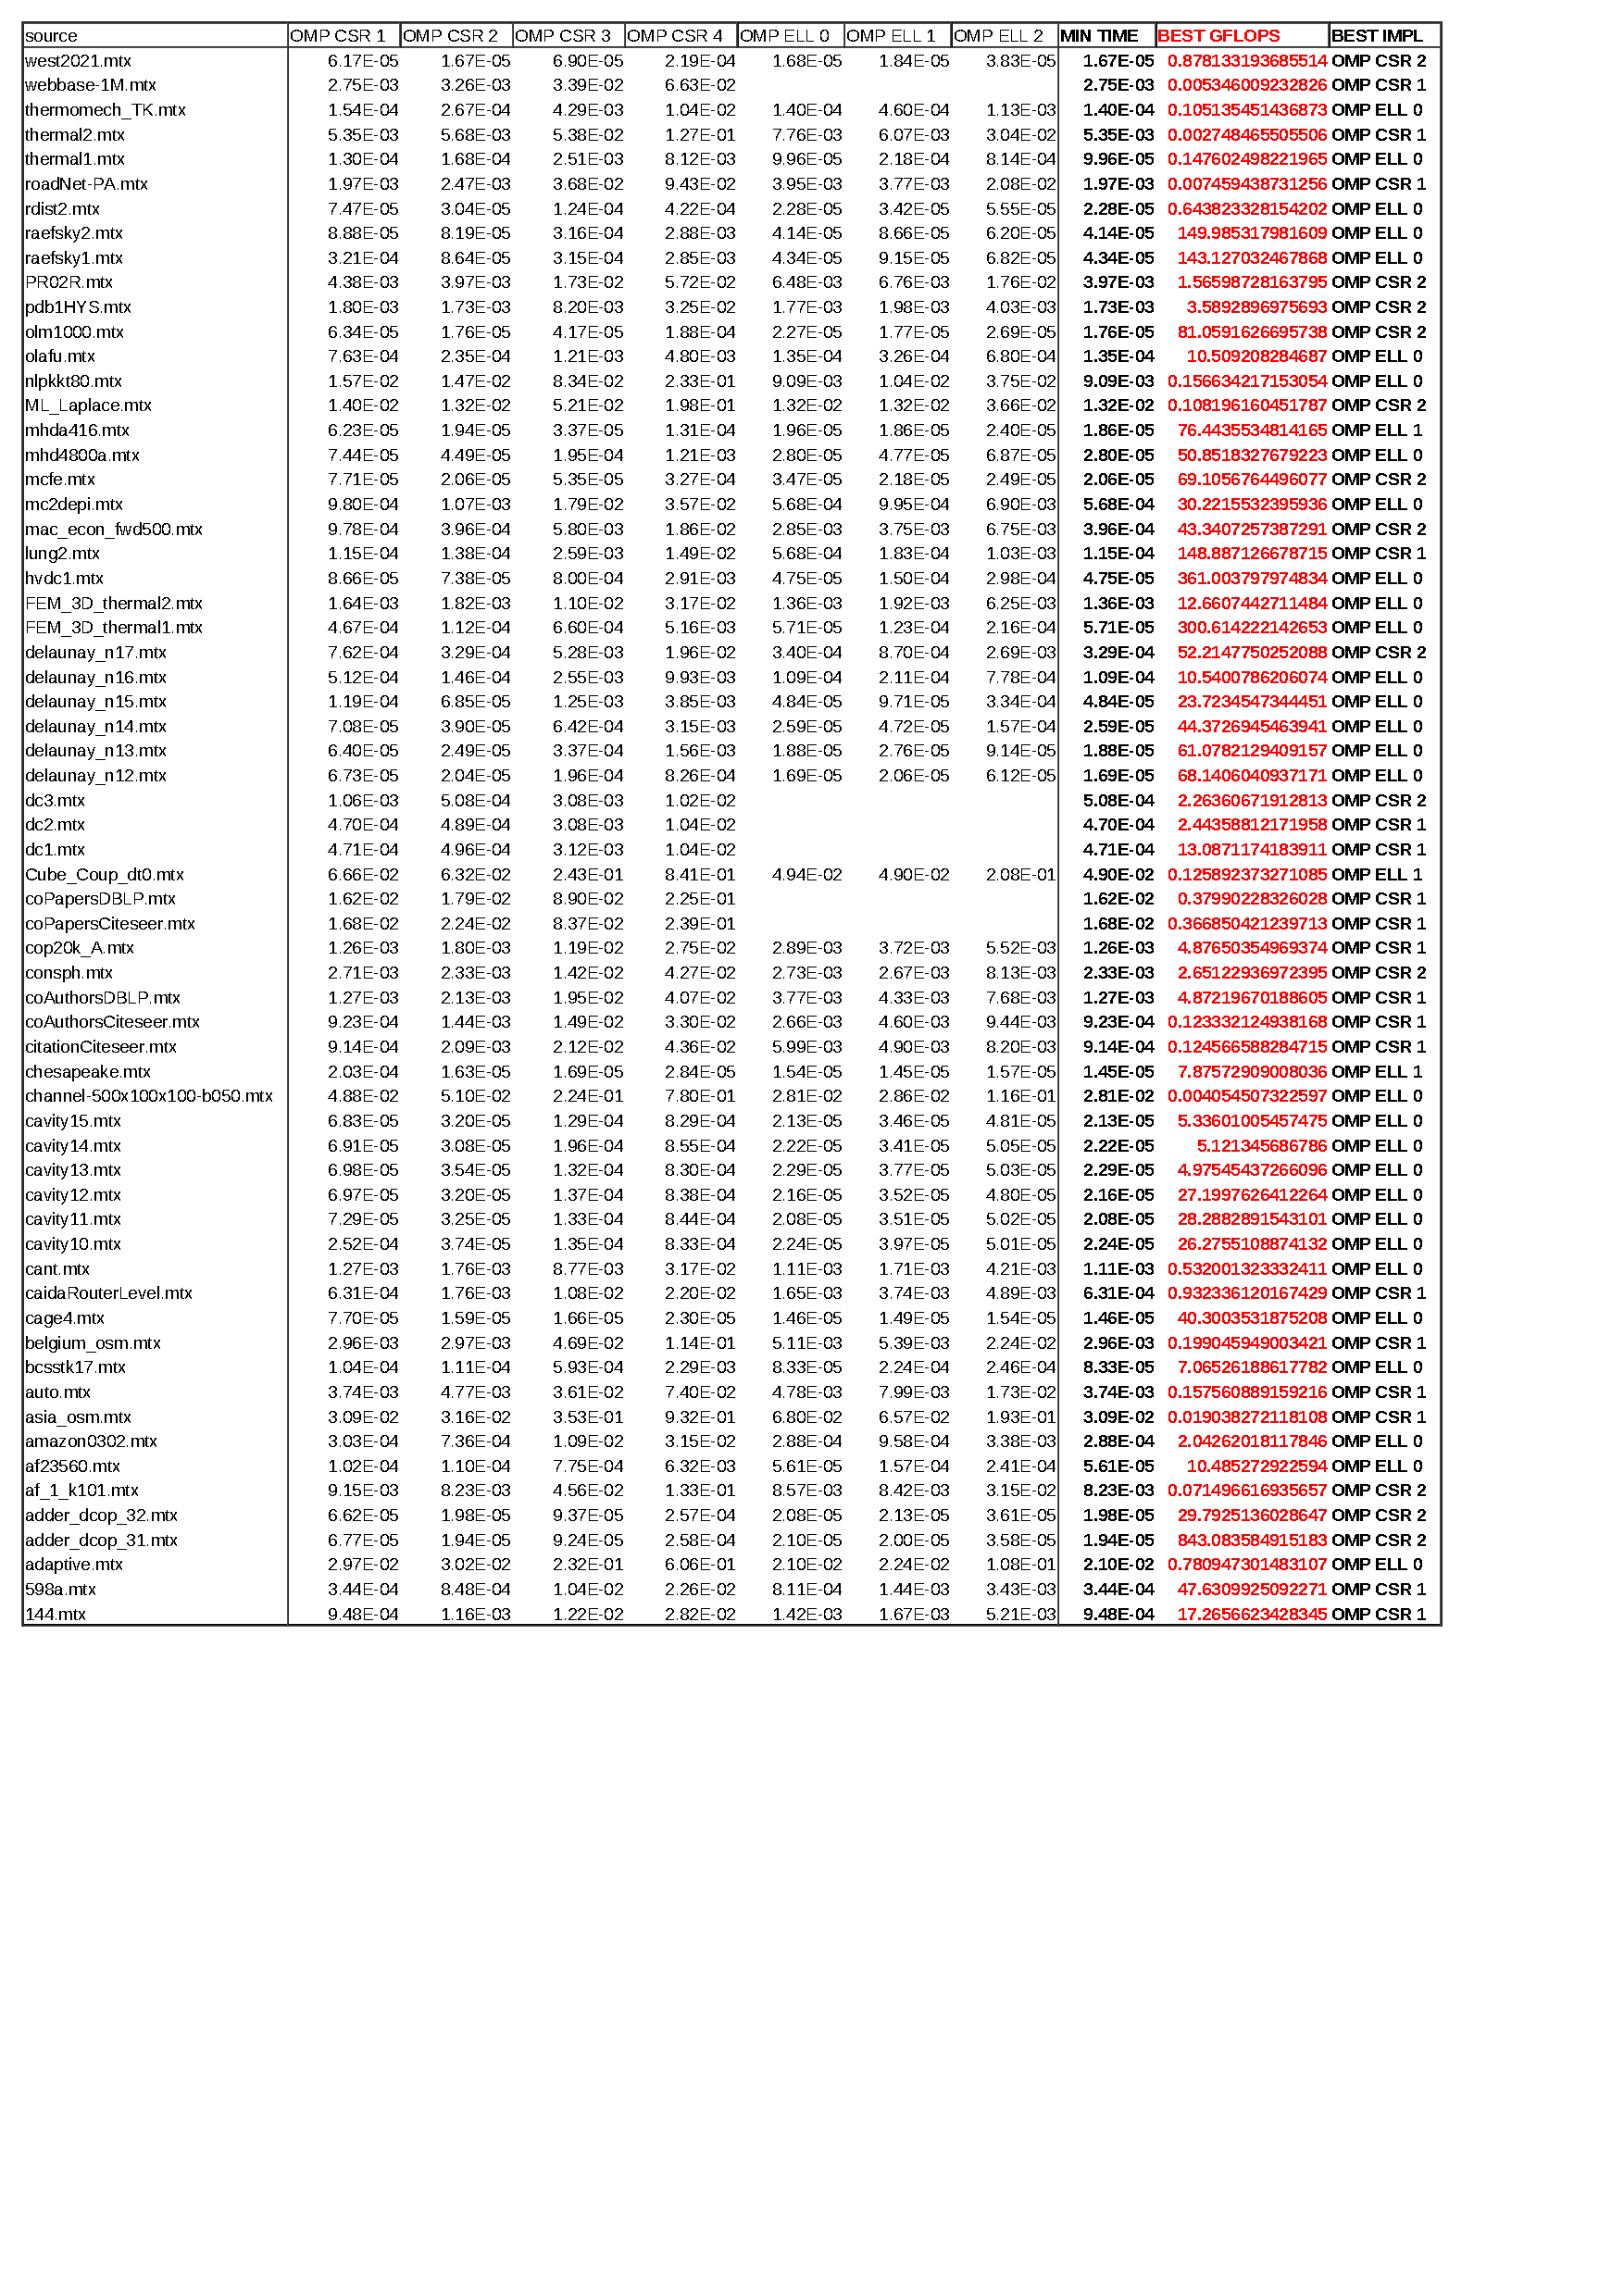
\includegraphics[scale=0.55]{ompNew_10x4_RL_NOSIMD_ImplConfrontoOut.pdf}
    \caption{performance implementazioni OpenMP}
\end{figure}

\clearpage

\subsection{Implementazioni CUDA}
\subsubsection{Configurazioni analizzate}
Le implementazioni confrontate sono:
\begin{itemize} 
 %matrici rappresentate in formato CSR
 \item CUDA CSR 0:	assegnamento di una riga CSR per thread
 \item CUDA CSR 1:	assegnamento di una riga CSR per warp

 %matrici rappresentate in formato ELL
 \item CUDA ELL 0:
	trasposizione della matrice ELL e assegnamento di una colonna per thread,
	come descritto in \ref{cudaSpMVRowsELL}
 \item CUDA ELL 1:
	assegnamento di una riga per thread, senza trasposizione
 \item CUDA ELL 2:
	assegnamento di una riga per warp senza trasposizione,
	come descritto in \ref{cudaSpMVWarpsPerRowELLNTrasposed}
\end{itemize}

Sono state confrontate inoltre:\\
\begin{itemize}
 \item l'utilizzo del vettore ausiliario \vvv{ROWLENS} per determinare la fine di ogni riga,\\
 \item 
	le seguenti configurazioni di blocchi per le implementazioni con assegnazione di 1 riga per thread:\\
	192 256 384
 \item 
	le seguenti configurazioni di blocchi per le implementazioni con assegnazione di 1 riga per warp:\\
	32x8 32x16 32x32
\end{itemize}

Seguono confronti con tutte le matrici in tutte le configurazioni dei blocchi
\subsubsection{Vettore ausiliario ROWLENS}
L'uso del vettore ausiliario ha creato uno svantaggio nel 55.96\% dei casi, 
senza dare significativi cambiamenti ai tempi di esecuzione.\\
Questo è probabilmente dovuto a questioni di divergenza tra i thread all'interno dello stesso warp.\\

\subsubsection{Configurazioni dei blocchi per il lancio dei kernel}
Le performance migliori sono state ottenute rispettivamente dalle configurazioni:\\
\begin{itemize}
 \item 192 e 32x8  nel 58.09\% dei casi
 \item 384 e 32x16 nel 34.32\% dei casi
 \item 256 e 32x32 nel  6.60\% dei casi
\end{itemize}


Segue un'analisi delle performance delle varie implementazioni CUDA, senza il vettore ausiliario ROWLENS
e con la configurazione di blocchi migliore: % \ref{cudaNoRowLens_192_8}

\begin{figure}[h] \label{cudaNoRowLens_192_8}
    \centering
    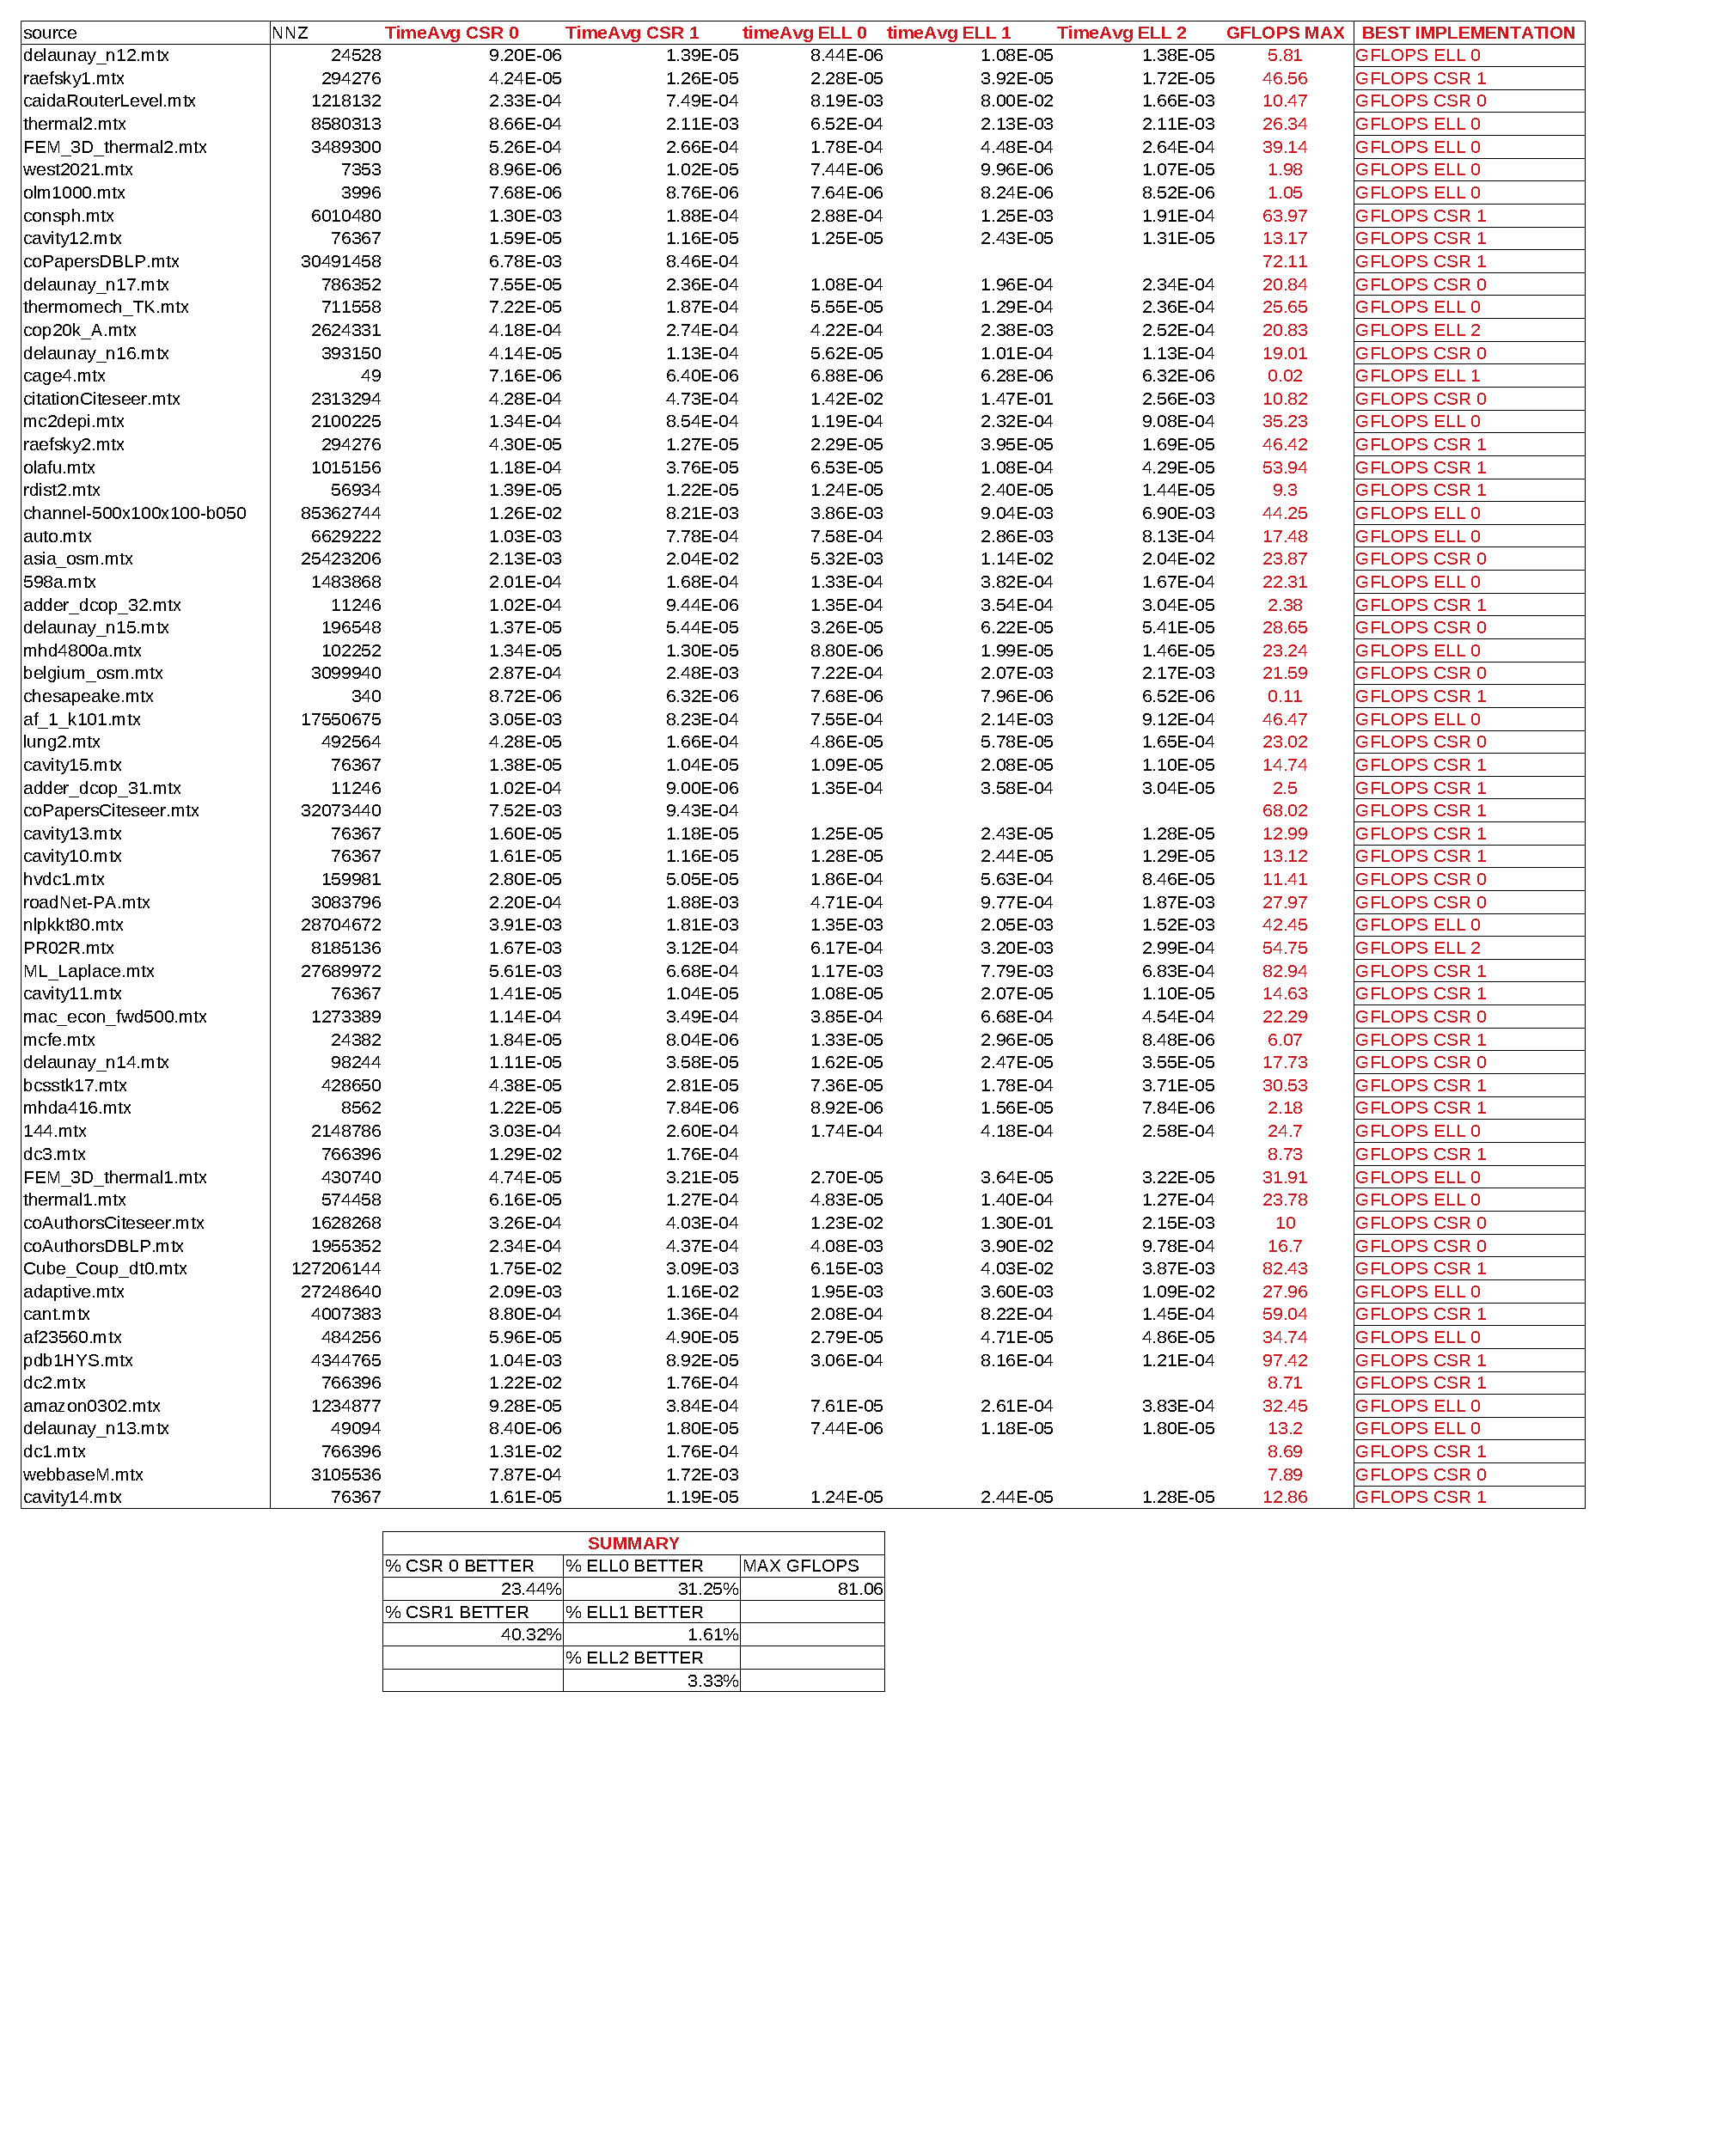
\includegraphics[scale=0.48]{cudaNoRowLens_192_8.pdf}
    \caption{performance implementazioni CUDA}
\end{figure}
\clearpage


\end{document}
\endinput	
